\documentclass{beamer}

\usetheme[secheader]{Madrid}

\usepackage{graphicx}
\graphicspath{ {./images/} }
\usepackage[table]{xcolor}

\usepackage{tikz}
\usetikzlibrary{shapes,arrows}
\usepackage[edges]{forest}
\usetikzlibrary{trees}


\newcommand{\highlight}[1]{{\color{blue} #1}}

\title{Segunda Reunión General del LMRI}
\subtitle{TIC: Unidad de Tecnologías de la Información y el Conocimiento}
\author[X. Campo]{Xandra Campo}
\institute[LMRI-CIEMAT]{Laboratorio de Metrología de Radiaciones Ionizantes (LMRI) \newline CIEMAT}
\date{9 de septiembre de 2024}

\begin{document}

	\maketitle

	\begin{frame}
		\frametitle{Table of Contents}
		\tableofcontents
	\end{frame}

	\section{Unidad de TIC}
	
	\subsection{Sobre la Unidad de TIC}
	
	\begin{frame}
		\frametitle{Sobre la Unidad de TIC}
		\framesubtitle{Cronología y organigrama}
		\begin{itemize}
			\item Unidad de \highlight{nueva creación}
			\item \highlight{Cronología}:
			\begin{itemize}
				\item Propuesta oficial en mayo de 2024
				\item Clave orgánica pendiente de asignación
				\item Clave funcional activa desde junio de 2024
				\item Trabajo activo desde febrero de 2024
			\end{itemize}
		\end{itemize}
		\bigskip
		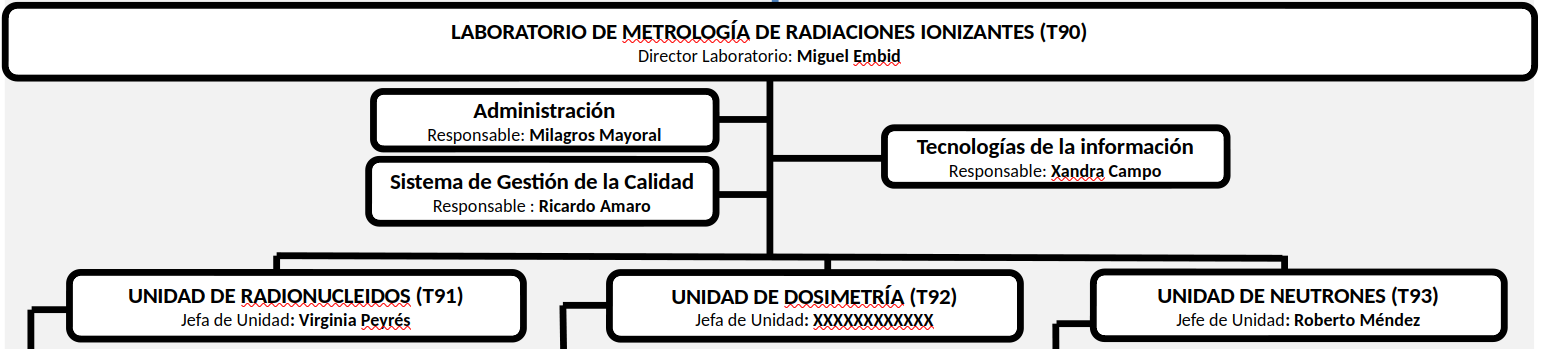
\includegraphics[width=\textwidth]{organigrama}
	\end{frame}
	
	\begin{frame}
		\frametitle{Sobre la Unidad de TIC}
		\framesubtitle{Objetivo y valores}
		\begin{itemize}
			\item \highlight{Objetivo}: Proporcionar soluciones de software y/o tecnologías asociadas que respondan a las necesidades del LMRI y los laboratorios que lo componen
			\item \highlight{Valores}:
			\begin{itemize}
				\item Uso y desarrollo de \highlight{software libre}
				\item \highlight{Recursos desarrollados públicos}: A nivel del LMRI o general, siempre que sea posible
				\item \highlight{Desarrollo compartido}: Metodologías de trabajo propias del desarrollo de software
			\end{itemize} 
			\item \highlight{Personal}: XCB y MES
		\end{itemize} 
	\end{frame}
	
	\begin{frame}
		\frametitle{Sobre la Unidad de TIC}
		\framesubtitle{Tipos de soluciones y metodologías de trabajo}
		\centering
		\rowcolors{2}{gray!15}{white}
		\begin{tabular}{ll}
			\rowcolor{blue!40}
			{\color{white}Tipos de soluciones}&{\color{white}Herramientas de desarrollo}\\
			Librerías de Python&Librerías de Python\\
			Scripts de Python&Librerías de Python\\
			Páginas web&Flask, Django\\
			Aplicaciones web&Flask, Django\\
			Aplicaciones de escritorio&Tkinter, PyQt\\
			Formación&Seminarios, cursos, prácticas\\
			\rowcolor{blue!40}
			{\color{white}Metodologías de trabajo}&{\color{white}Herramientas de desarrollo}\\
			Entornos de trabajo&PyCharm, Git, GitHub\\
			Plataformas de difusión&GitHub, PyPI\\
		\end{tabular}
	\end{frame}
	
	\subsection{Resumen de actividades}
	
	\begin{frame}
		\frametitle{Resumen de actividades}
		\centering
		\highlight{Total}: 22 proyectos de febrero a agosto de 2024 (7 meses)
		\begin{columns}
			\begin{column}{0.35\textwidth}
				\begin{block}{Estado del proyecto}
					\begin{tabular}{ll}
						Mantenimiento&12\\
						En desarrollo&5\\
						Pendiente&5\\
					\end{tabular}
				\end{block}
				\begin{block}{Área de aplicación}
					\begin{tabular}{ll}
						GuideRadPROS&9\\
						IR14D&5\\
						LMRI&5\\
						IR13&2\\
						IR14F&1\\
					\end{tabular}
				\end{block}
			\end{column}
			\begin{column}{0.35\textwidth}
				\begin{block}{Visibilidad del proyecto}
					\begin{tabular}{ll}
						Pública&11\\
						Privada&11\\
					\end{tabular}
				\end{block}
				\begin{block}{Tipo de solución}
					\begin{tabular}{ll}
						Librerías Python&6\\
						Aplicaciones&6\\
						Sitios Web&2\\
						Scripts&2\\
						Otros&2\\
						Formación&4\\
					\end{tabular}
				\end{block}
			\end{column}
		\end{columns}
	\end{frame}
	
	\subsection{Proyectos}
		
	\begin{frame}
		\frametitle{Proyectos}
		\framesubtitle{EURAMET GuideRadPROS project}
		\centering
		\small
		\begin{forest}
			forked edges,
			for tree={
				%grow=0,
				rounded corners,
				fill=blue!20,
				edge={-latex},
				align=center,
			}
			[GuideRadPROS Project
				[Página web\\del proyecto, fill=green!20,
					[Practicas\\estudiante\\FP, fill=green!20]
				]
				[Librería USpekPy, fill=green!20
					[Aplicación\\web
						[Practicas\\estudiante\\FP, fill=red!20]
					]
					[Seminario\\uso\\librería, fill=green!20]
					[Script\\ficheros\\entrada, fill=green!20]
					[Script\\análisis\\librería, fill=green!20]
					[Publicar\\librería\\SpekPy, fill=green!20]
				]
			]
		\end{forest}
	\end{frame}
	
	\begin{frame}
		\frametitle{Proyectos}
		\framesubtitle{EURAMET GuideRadPROS project: Página web}
		\begin{itemize}
			\item Necesidad: 
			\begin{itemize}
				\item CIEMAT es responsable de poner en marcha la \highlight{web oficial del proyecto}.
				\item Las limitaciones en el desarrollo y mantenimiento de la web en CIEMAT son muy altas.
			\end{itemize}
			\item Solución:
			\begin{itemize}
				\item \highlight{Diseño y desarrollo} de nueva web con herramientas gratuitas y modernas (Flask)
				\item Esto también facilita mucho el \highlight{mantenimiento} de la web
				\item \highlight{Alojamiento}: GitHub Pages. Gratuito pero no ideal
			\end{itemize}
			\item Colaboración: XCB, PAL, CGM, MBR, estudiante de FP en prácticas.
		\end{itemize}
	\end{frame}
	
	\begin{frame}
		\frametitle{Proyectos}
		\framesubtitle{EURAMET GuideRadPROS project: Página web}
		\centering
		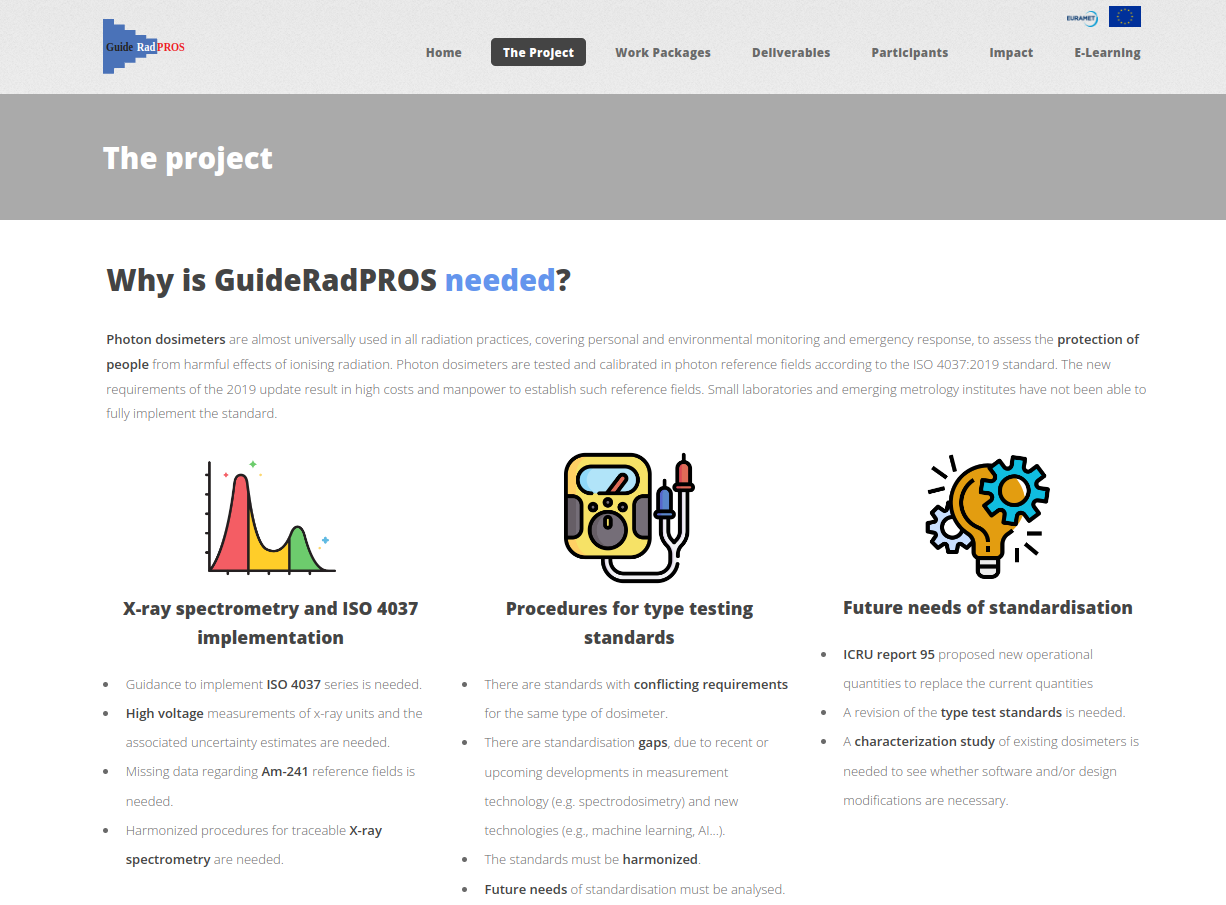
\includegraphics[width=\textwidth]{GRP_website}
	\end{frame}
	
	\begin{frame}
		\frametitle{Proyectos}
		\framesubtitle{EURAMET GuideRadPROS project: Librería USpekPy}
		\begin{itemize}
			\item Necesidad: 
			\begin{itemize}
				\item \highlight{Actividades CIEMAT}: calculo de incertidumbres en magnitudes integrales de espectros de rayos x simulados mediante Monte Carlo
				\item Mejor forma: mediante algoritmos
			\end{itemize}
			\item Soluciones:
			\begin{itemize}
				\item \highlight{Script PAL}: diseño, desarrollo y publicación de librería de Python: provee las herramientas necesarias para los cálculos
				\item Basada en \highlight{SpekPy}: Se publica y mantiene actualizada en PyPI
				\item Desarrollo de herramientas a partir de la librería para facilitar su uso
				\item \highlight{Scripts}: calculo de incertidumbres, generar ficheros de entrada, analizar el comportamiento de la librería
				\item \highlight{Aplicación web}: Facilitar el uso a quien no programan en Python
				\item \highlight{Seminario online} sobre su uso: para los socios del proyecto, uno antes del verano y otro después
			\end{itemize}
			\item Colaboración: XCB, PAL
		\end{itemize}
	\end{frame}
	
	\begin{frame}
		\frametitle{Proyectos}
		\framesubtitle{EURAMET GuideRadPROS project: Librería USpekPy}
		\centering
		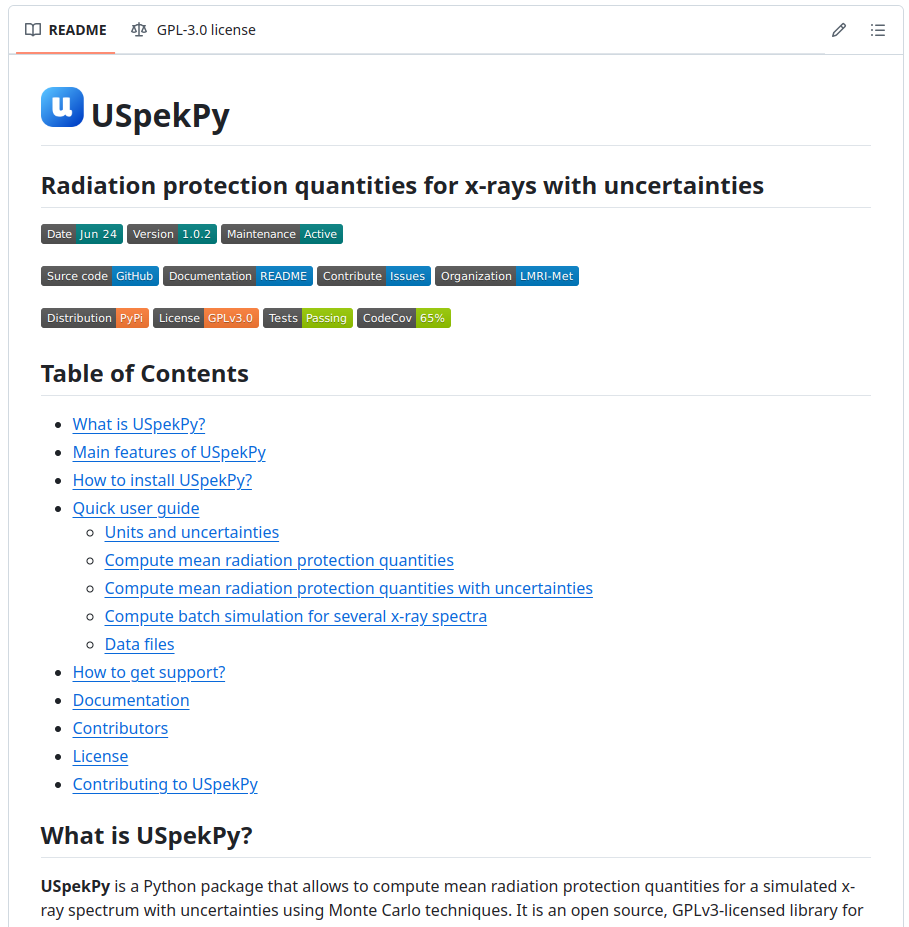
\includegraphics[width=\textwidth]{GRP_uspekpy}
	\end{frame}
	
	\begin{frame}
		\frametitle{Proyectos}
		\framesubtitle{EURAMET GuideRadPROS project: Librería SPekPy}
		\centering
		\begin{columns}[T]
			\begin{column}{0.55\textwidth}
				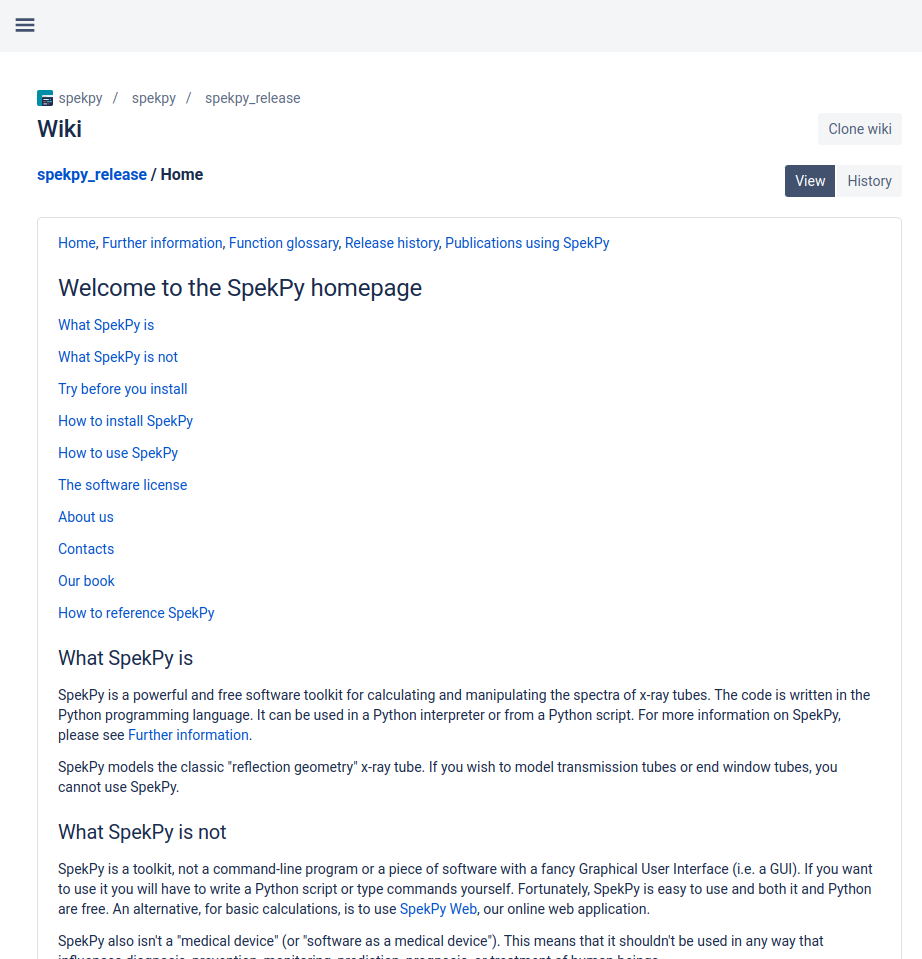
\includegraphics[width=\textwidth]{GRP_spekpy_bitbucket}
			\end{column}
			\begin{column}{0.4\textwidth}
				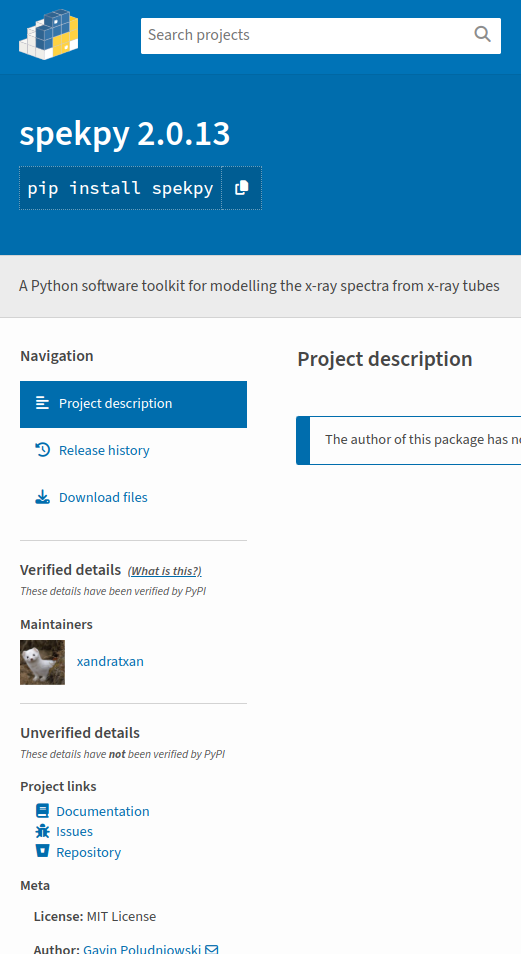
\includegraphics[width=\textwidth]{GRP_spekpy}
			\end{column}
		\end{columns}
	\end{frame}
	
	\begin{frame}
		\frametitle{Proyectos}
		\framesubtitle{EURAMET GuideRadPROS project: Seminario USpekPy}
		\centering
		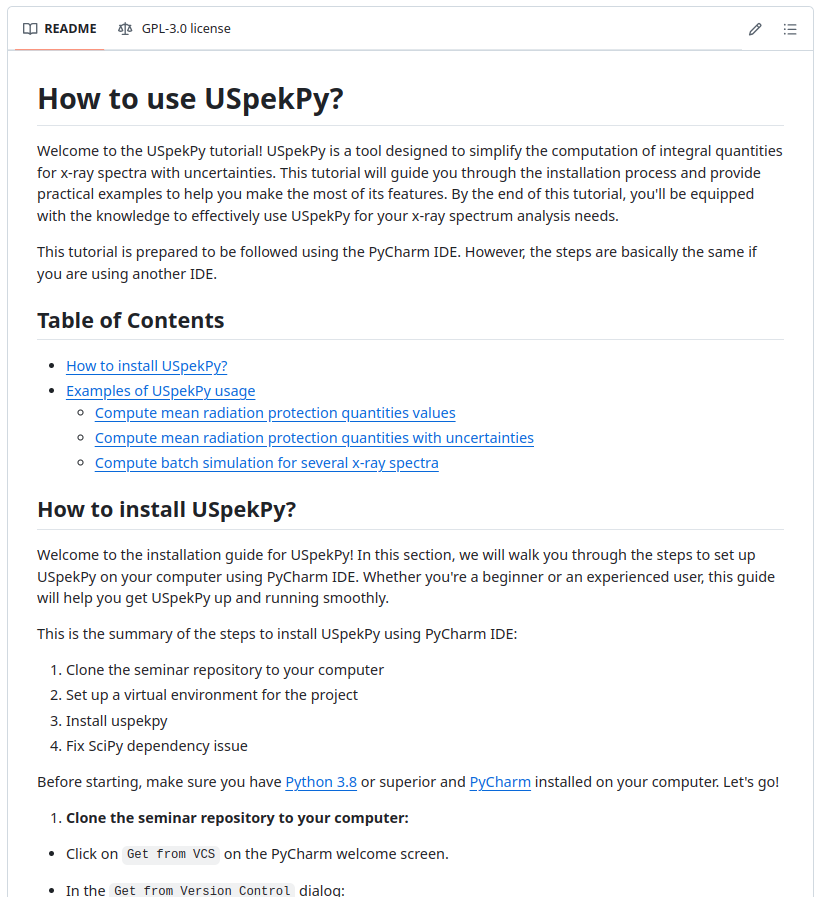
\includegraphics[width=\textwidth]{GRP_seminar}
	\end{frame}
	
	\begin{frame}
		\frametitle{Proyectos}
		\framesubtitle{EURAMET GuideRadPROS project: Scripts}
		\centering
		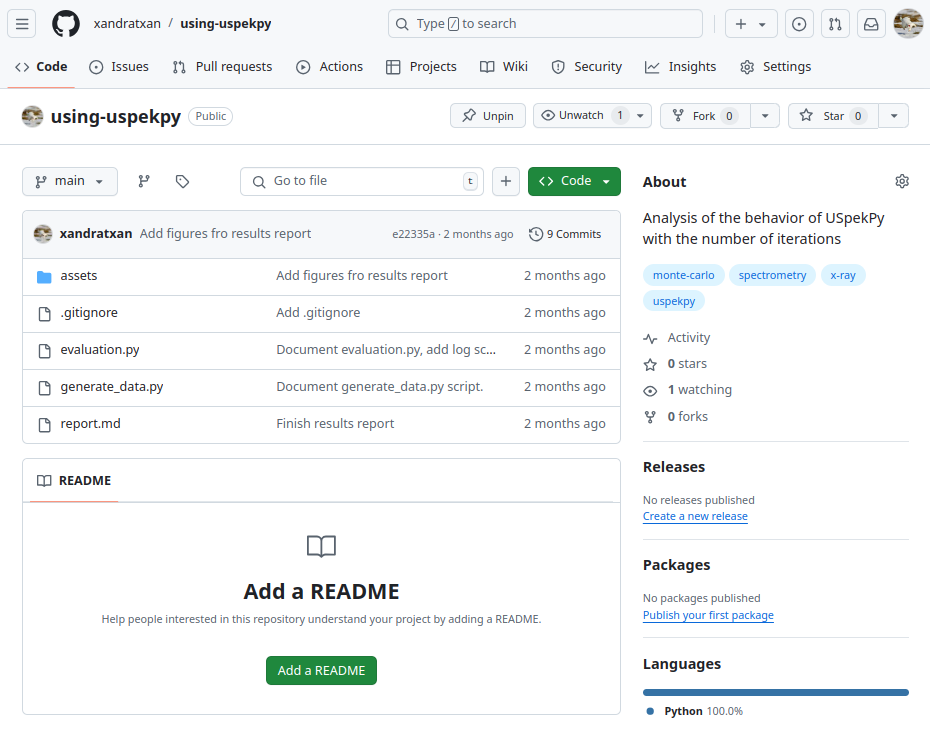
\includegraphics[width=\textwidth]{GRP_analisis}
	\end{frame}
	
	\begin{frame}
		\frametitle{Proyectos}
		\framesubtitle{EURAMET GuideRadPROS project: Scripts}
		\centering
		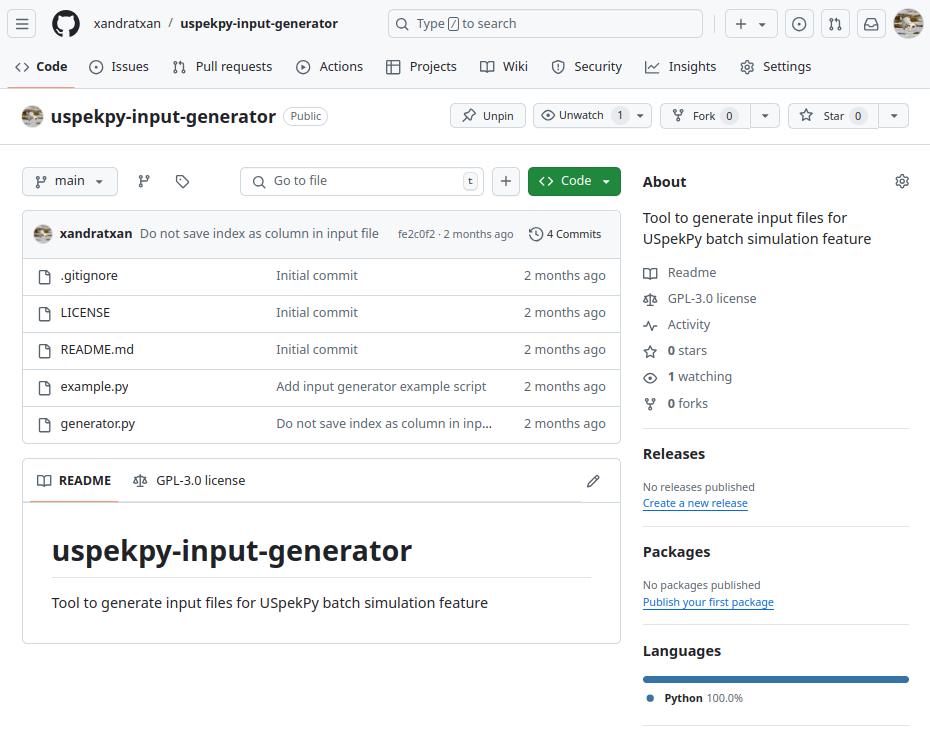
\includegraphics[width=\textwidth]{GRP_input}
	\end{frame}
	
	\begin{frame}
		\frametitle{Proyectos}
		\framesubtitle{IR14-D: Patrones dosimétricos de rayos X}
		\centering
		\small
		\begin{forest}
			forked edges,
			for tree={
				%grow=0,
				rounded corners,
				fill=blue!20,
				edge={-latex},
				align=center,
			}
			[IR14-D
				[Librería\\espectrometría, fill=red!20]
				[Librería\\MetPyX, fill=green!20]
				[Librería automatización\\cadena medida
					[Aplicación web o de escritorio]
				]
				[Aplicación\\lectura barómetro, fill=green!20]
			]
		\end{forest}
	\end{frame}
	
	\begin{frame}
		\frametitle{Proyectos}
		\framesubtitle{IR14-D: Patrones dosimétricos de rayos X}
		Renovación completa del laboratorio de rayos x
		\begin{itemize}
			\item Necesidad:
			\begin{itemize}
				\item Puesta en marcha del laboratorio
				\item Caracterización de los haces de rayos x (\highlight{espectrometría} experimental)
				\item \highlight{Digitalización} de la cadena de medida
				\item \highlight{Automatización} de calibraciones y asignaciones de dosis
			\end{itemize}
			\item Solución:
			\begin{itemize}
				\item Desarrollo de \highlight{librerías} básicas
				\item Desarrollo de \highlight{herramientas asociadas} (scripts, aplicaciones)
			\end{itemize}
			\item Colaboración: XCB, MES, MBR
		\end{itemize}
	\end{frame}
	
	\begin{frame}
		\frametitle{Proyectos}
		\framesubtitle{IR14-D: Librería MetPyX}
		\centering
		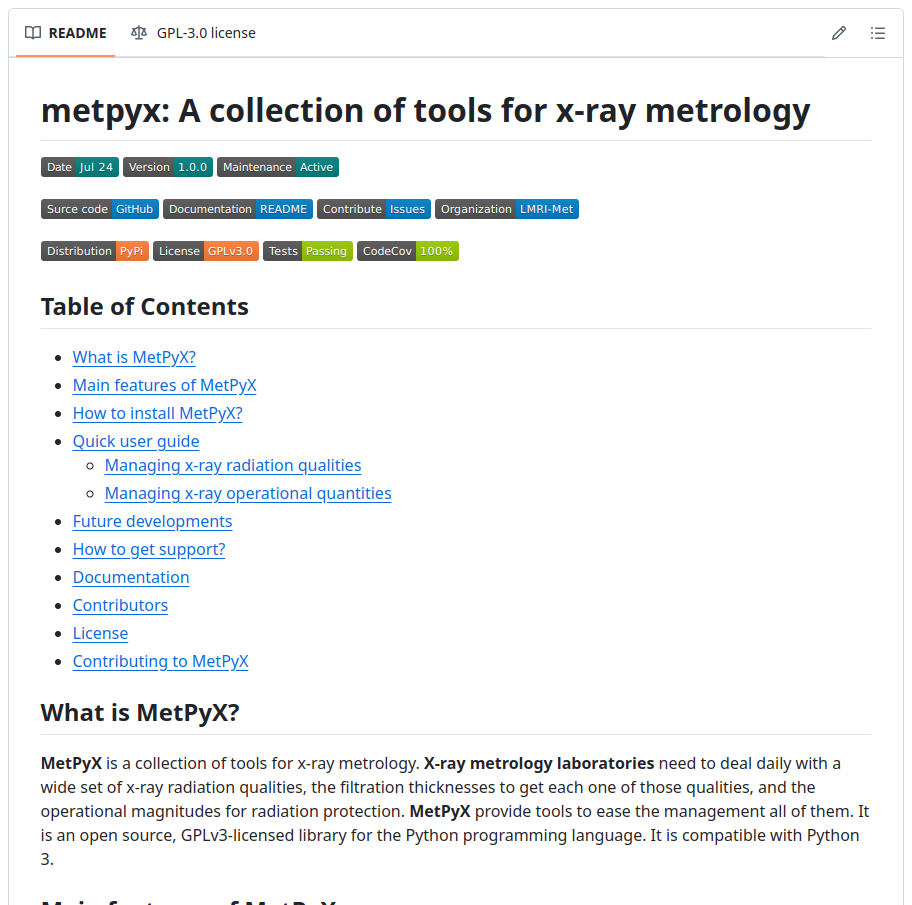
\includegraphics[width=\textwidth]{IR14D_metpyx}
	\end{frame}
	
	\begin{frame}
		\frametitle{Proyectos}
		\framesubtitle{IR14-D: Aplicación automatización cadena medida}
		\centering
		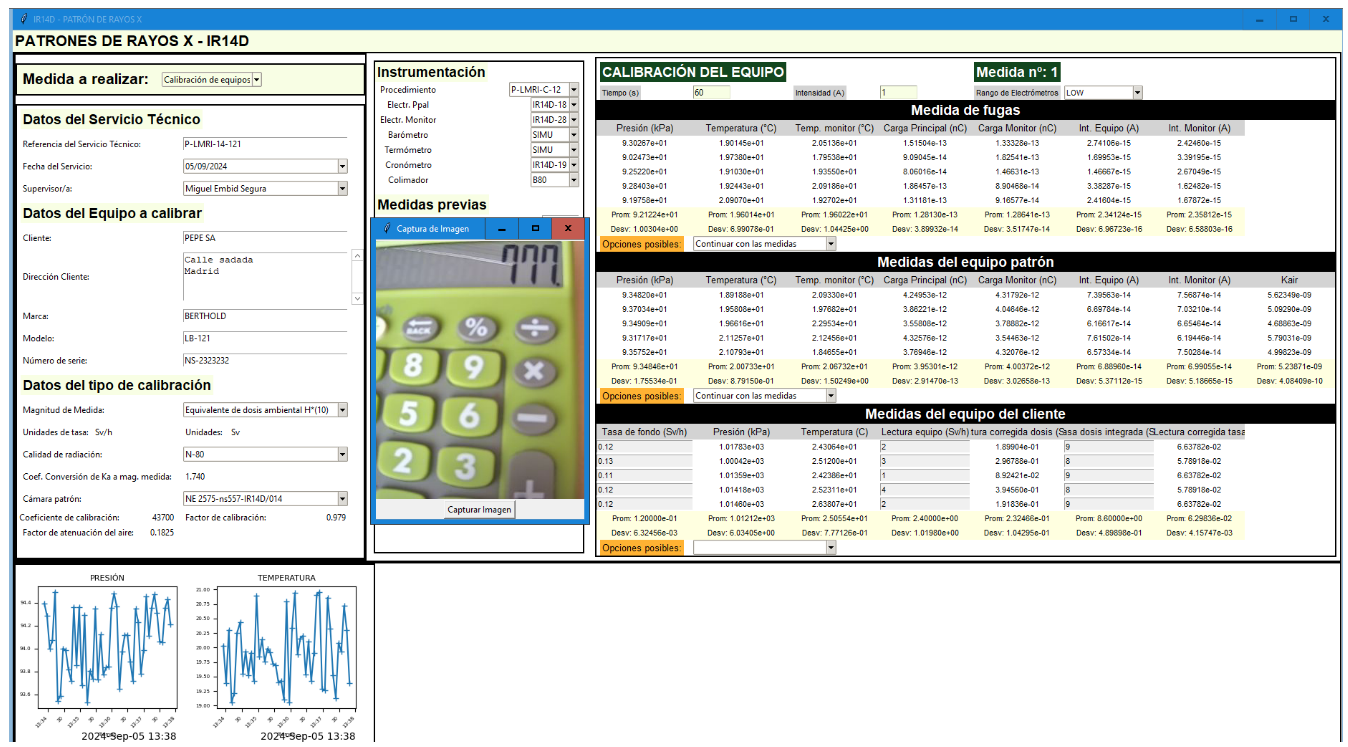
\includegraphics[width=\textwidth]{IR14D_app_automatizacion}
	\end{frame}
	
	\begin{frame}
		\frametitle{Proyectos}
		\framesubtitle{IR14-D: Patrones dosimétricos de rayos X}
		Aplicación lectura barómetro
		\begin{itemize}
			\item Necesidad:
			\begin{itemize}
				\item Se manda a calibrar al CEM un \highlight{barómetro}
				\item No pueden leer el equipo: aplicación para \highlight{Windows XP}
			\end{itemize}
			\item Solución:
			\begin{itemize}
				\item Desarrollo de \highlight{aplicación de escritorio} que el CEM usa como monitor
			\end{itemize}
			\item Autor: MES
		\end{itemize}
	\end{frame}
	
	\begin{frame}
		\frametitle{Proyectos}
		\framesubtitle{IR14-D: Aplicación lectura barómetro MetPyX}
		\centering
		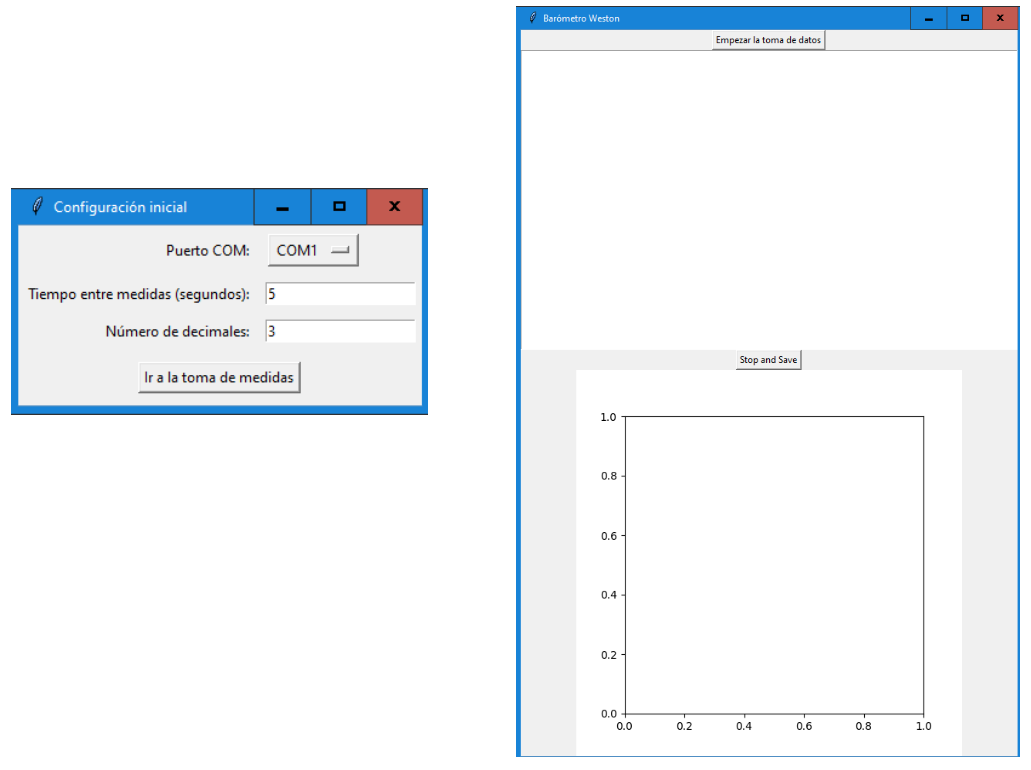
\includegraphics[width=0.7\textwidth]{IR14D_barometro}
	\end{frame}
	
	\begin{frame}
		\frametitle{Proyectos}
		\framesubtitle{LMRI e IR13}
		\centering
		\small
		\tikzstyle{every node}=[rounded corners,fill=blue!20,anchor=west]
		\tikzstyle{completed}=[fill=green!20]
		\tikzstyle{todo}=[fill=red!20]
		\begin{columns}
			\begin{column}{0.45\textwidth}
				\begin{tikzpicture}[
					grow via three points={one child at (0.5,-0.7) and two children at (0.5,-0.7) and (0.5,-1.4)},
					edge from parent path={(\tikzparentnode.south) |- (\tikzchildnode.west)}
					]
					\node {LMRI}
					child { node [completed] {Organización de GitHub}}
					child { node {Servidor web LMRI}}		
					child { node {Página web LMRI}}
					child { node [todo] {Librería cálculo incertidumbres}}
					child [missing] {}
					child { node [todo, align=left] {Curso ecosistema \\de trabajo de Pyhton}}
					;
				\end{tikzpicture}
			\end{column}
			\begin{column}{0.45\textwidth}
				\begin{tikzpicture}[
					grow via three points={one child at (0.5,-0.7) and two children at (0.5,-0.7) and (0.5,-1.4)},
					edge from parent path={(\tikzparentnode.south) |- (\tikzchildnode.west)}
					]
					\node {IR13}
					child { node [completed, align=left] {Aplicación cámara IG11:\\SIR}}
					child [missing] {}
					child { node [completed, align=left] {Aplicación cámara IG11:\\Series temporales}}
					;
				\end{tikzpicture}
			\end{column}
		\end{columns}
	\end{frame}
	
	\begin{frame}
		\frametitle{Proyectos}
		\framesubtitle{LMRI}
		Organización de GitHub
		\begin{itemize}
			\item \highlight{Repositorio} centralizado y compartido de código para el LMRI
			\item Fomentar el \highlight{desarrollo compartido} y las metodologías de trabajo propias del desarrollo de software
		\end{itemize}
		Curso ecosistema de trabajo de Pyhton
		\begin{itemize}
			\item \highlight{Metodologías de trabajo} propias del desarrollo de software (control de versiones, desarrollo compartido)
			\item \highlight{Herramientas} gratuitas y disponibles para ello asociadas a Python (Pycharm, Git, GitHub)
		\end{itemize}
	\end{frame}
	
	\begin{frame}
		\frametitle{Proyectos}
		\framesubtitle{LMRI: Organización en GitHub}
		\centering
		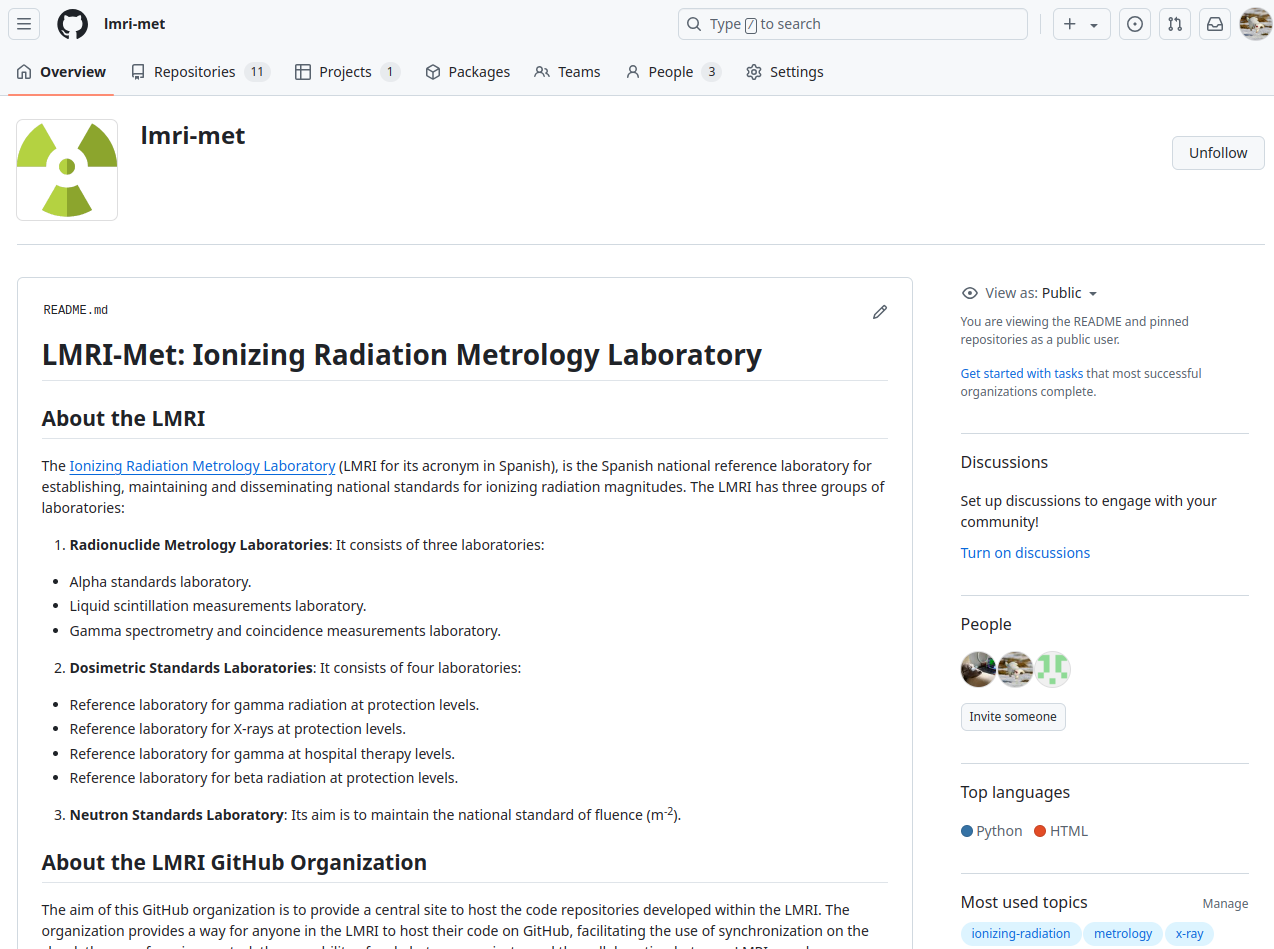
\includegraphics[width=\textwidth]{LMRI_github_org}
	\end{frame}
	
	\begin{frame}
		\frametitle{Proyectos}
		\framesubtitle{LMRI}
		Página web LMRI
		\begin{itemize}
			\item \highlight{Modernización} de la web del LMRI
			\item Automatización de la solicitud de \highlight{servicios técnicos}
		\end{itemize}
		Servidores web LMRI
		\begin{itemize}
			\item Solución de \highlight{alojamiento} para las paginas y aplicaciones web desarrolladas en el LMRI
			\item \highlight{Servidor} externo (XCB) e interno (TIC) 
		\end{itemize}
	\end{frame}
	
	\begin{frame}
		\frametitle{Proyectos}
		\framesubtitle{LMRI: Página web LMRI con formulario para servicios técnicos}
		\centering
		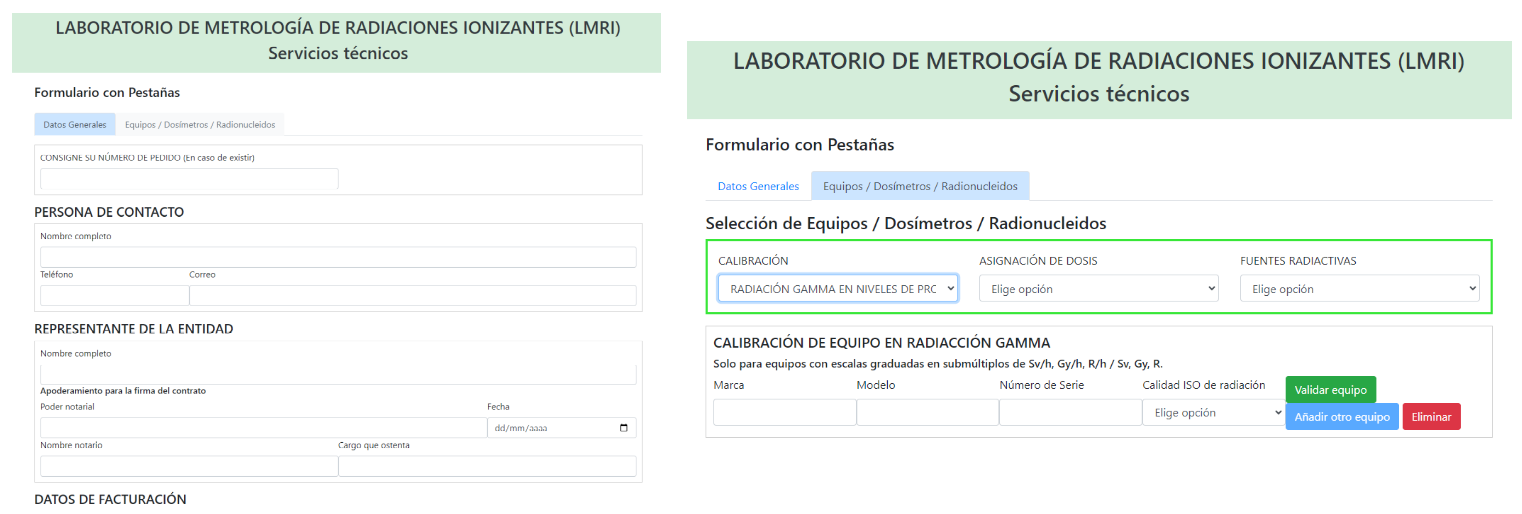
\includegraphics[width=\textwidth]{LMRI_servicios_tecnicos}
	\end{frame}
	
	\begin{frame}
		\frametitle{Proyectos}
		\framesubtitle{IR13}
		Aplicaciones para cámara de ionización IG11
		\begin{itemize}
			\item Aplicación del equipo sólo corre en \highlight{sistemas operativos antiguos}
			\item Desarrollo de dos \highlight{aplicaciones de escritorio} para:
			\begin{itemize}
				\item Calibración y cálculo de actividad de muestras de emisores gamma
				\item Medidas del tiempo de decaimiento de muestras de emisores gamma
			\end{itemize}
		\end{itemize}
	\end{frame}
	
	\begin{frame}
		\frametitle{Proyectos}
		\framesubtitle{IR13: Aplicación para cámara IG11: SIR}
		\centering
		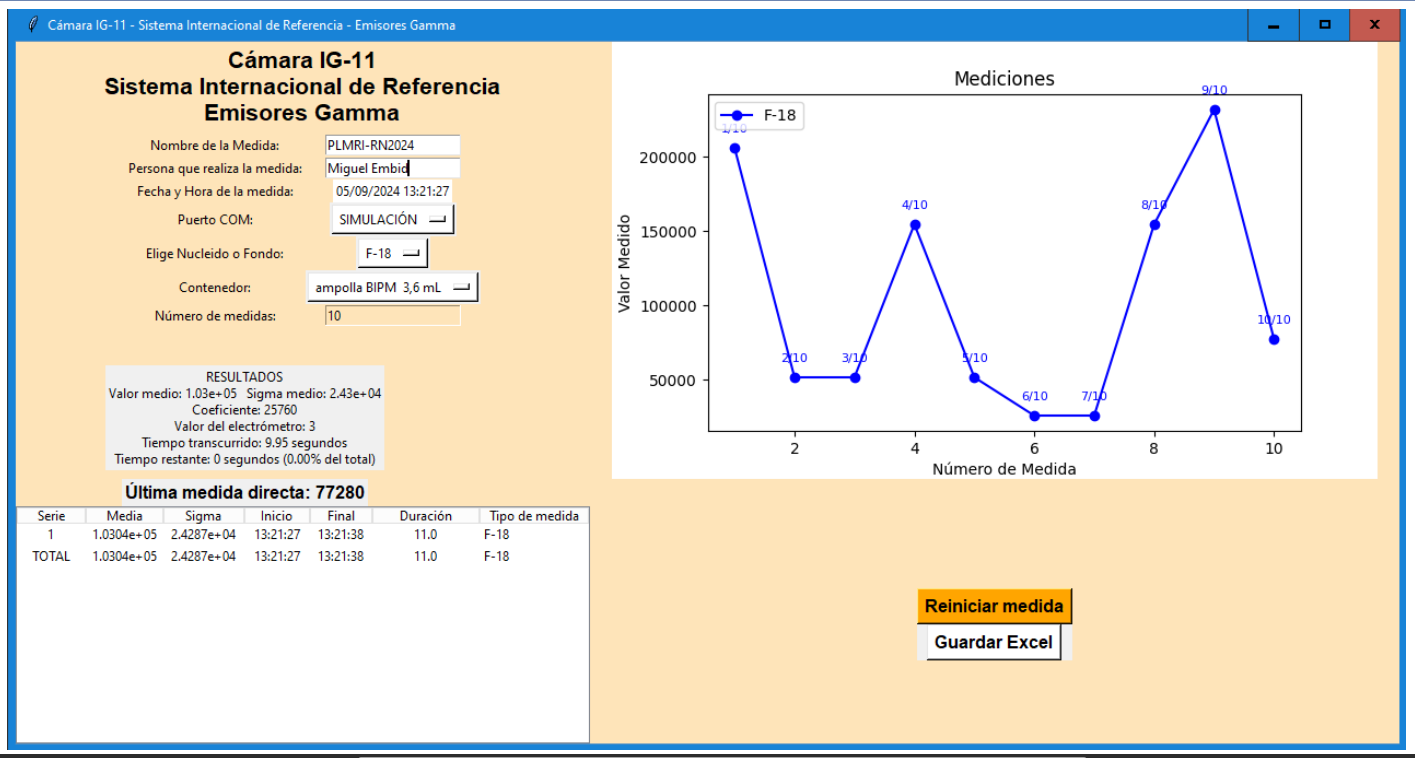
\includegraphics[width=\textwidth]{IR13_SIR}
	\end{frame}
	
	\begin{frame}
		\frametitle{Proyectos}
		\framesubtitle{IR13: Aplicación para cámara IG11: Series temporales}
		\centering
		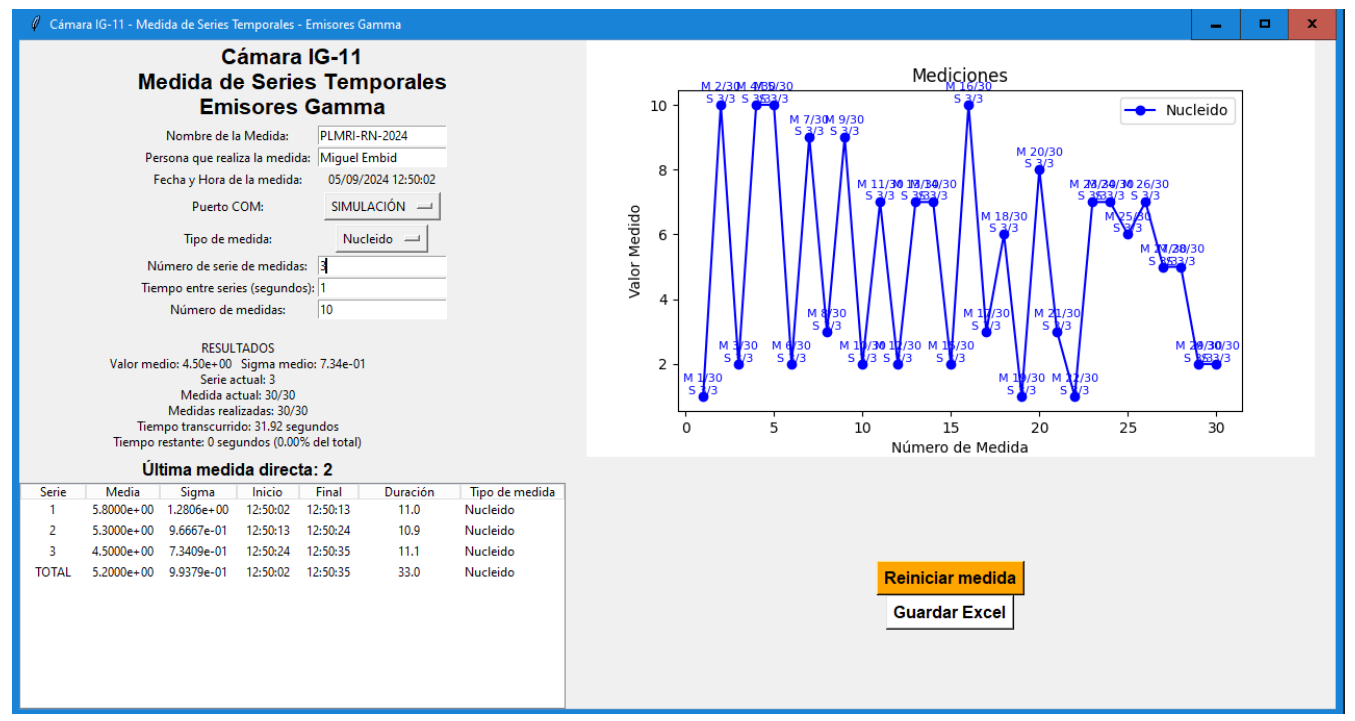
\includegraphics[width=\textwidth]{IR13_series_temporales}
	\end{frame}
	
	\begin{frame}
		\frametitle{Proyectos}
		\framesubtitle{Herramientas públicas: enlaces de interés}
		\centering
		\scriptsize
		\rowcolors{2}{gray!15}{white}
		\begin{tabular}{ll}			
			\rowcolor{blue!40}
			{\color{white}GuideRadPROS}&\\
			Web del proyecto&https://github.com/lmri-met/sites-guideradpros\\
			&https://lmri-met.github.io/sites-guideradpros/\\
			USpekPy: Librería&https://github.com/lmri-met/uspekpy\\
			USpekPy: Seminario&https://github.com/xandratxan/uspekpy-seminar\\
			USpekPy: Análisis librería&https://github.com/xandratxan/using-uspekpy\\
			USpekPy: Generador input&https://github.com/xandratxan/uspekpy-input-generator\\
			USpekPy: Aplicación web&https://github.com/lmri-met/uspekpy-web\\
			SpekPy: Librería&https://pypi.org/project/spekpy/\\
			\rowcolor{blue!40}
			{\color{white}IR14-D}&\\
			MetPyX: Librería&https://github.com/lmri-met/metpyx\\
			\rowcolor{blue!40}
			{\color{white}LMRI}&\\
			Organización del LMRI en GitHub&https://github.com/lmri-met\\
			Librería incertidumbres&https://github.com/xandratxan/physical-magnitude\\
		\end{tabular}
	\end{frame}
	
	\subsection{Objetivos}
	
	\begin{frame}
		\frametitle{Objetivos}
		\framesubtitle{Segundo semestre 2024}
		\begin{itemize}
			\item \highlight{Mantenimiento} de las herramientas ya desarrolladas
			\item \highlight{GuideRadPROS}: 
			\begin{itemize}
				\item Aplicación web USekPy
				\item Seminario librería USpekPy
			\end{itemize}
			\item \highlight{IR14-D}:
			\begin{itemize}
				\item Librería y scripts/aplicación para espectrometría experimental
				\item Librería y aplicación para automatizar la cadena medida 
			\end{itemize}
			\item \highlight{LMRI}:
			\begin{itemize}
				\item Puesta en marcha servidor web
				\item Formación en el ecosistema de Python
			\end{itemize}
		\end{itemize}
	\end{frame}
	
	\subsection{Necesidades}
	
	\begin{frame}
		\frametitle{Necesidades}
		¿Solución para poder \highlight{hospedar páginas y aplicaciones}?
		\begin{itemize}
			\item ¿Alquiler de espacio en servidor web comercial?
			\item ¿Puesta en marcha de nuestro propio servidor?
			\item ¿Otras opciones en Ciemat fuera de las oficiales?
		\end{itemize}
		Páginas y aplicaciones web \highlight{públicas}:
		\begin{itemize}
			\item Puesta en marcha de servidor web externo a CIEMAT
			\item Recursos propios de XCB
		\end{itemize}
		Páginas y aplicaciones web para el \highlight{LMRI}:		
		\begin{itemize}
			\item Puesta en marcha de un servidor web interno
			\item Sería necesario un ordenador + monitor
		\end{itemize}		
	\end{frame}
	
	\subsection{}
	
	\begin{frame}
		\begin{block}{}
			\centering
			¡Gracias por vuestra atención!
		\end{block}
	\end{frame}

\end{document}

%	\begin{frame}
	%		% Define block styles
	%		
	%		\tikzstyle{block} = [
	%		rectangle,
	%		rounded corners,
	%		fill=blue!20,
	%		%draw, % Contour line
	%		%text width=7em, % Width
	%		text centered,
	%		%minimum height=4em
	%		node distance=3cm,
	%		%inner sep=0pt
	%		]
	%		
	%		\tikzstyle{line} = [
	%		draw, 
	%		-latex' % Arrow
	%		]
	%		
	%		\begin{tikzpicture}[
		%			%node distance = 3cm, 
		%			auto
		%			]
		%			% Place nodes
		%			\node [block] (spekpy) {SpekPy};
		%			\node [block, below of=spekpy] (uspekpy) {USpekPy};
		%			\node [block, left of=uspekpy, align=center] (ficheros) {Generador\\ficheros\\entrada};
		%			\node [block, right of=uspekpy, align=center] (análisis) {Análisis\\comportamiento};
		%			\node [block, below of=uspekpy, align=center] (aplicación) {Aplicación\\web};
		%			\node [block, left of=aplicación, align=center] (seminario) {Seminario\\uso librería};
		%			\node [block, right of=aplicación, align=center] (estudiante2) {Estudiante\\prácticas};
		%		
		%			% Draw edges
		%			\path [line] (spekpy) -- (uspekpy);
		%			\path [line] (uspekpy) -- (seminario);
		%			\path [line] (uspekpy) -- (ficheros);
		%			\path [line] (uspekpy) -- (análisis);
		%			\path [line] (uspekpy) -- (aplicación);
		%			\path [line] (estudiante2) -- (aplicación);
		%		\end{tikzpicture}
	%	\end{frame}
%	
%\begin{frame}
%	% Define block styles
%	
%	\tikzstyle{block} = [
%	rectangle,
%	rounded corners,
%	fill=blue!20,
%	%draw, % Contour line
%	text width=5em, % Width
%	text centered,
%	%minimum height=4em
%	%node distance=3cm,
%	%inner sep=0pt
%	]
%	
%	\tikzstyle{line} = [
%	draw, 
%	-latex' % Arrow,
%	forked edges
%	]
%	
%	\begin{tikzpicture}[
	%		node distance = 2cm, 
	%		auto
	%		]
	%		% Place nodes
	%		\node [block] (spekpy) {SpekPy};
	%		\node [block, below of=spekpy] (uspekpy) {USpekPy};
	%		\node [block, right of=spekpy, align=center] (ficheros) {Generador ficheros entrada};
	%		\node [block, right of=uspekpy, align=center] (análisis) {Análisis comportamiento};
	%		\node [block, below of=análisis, align=center] (aplicación) {Aplicación web};
	%		\node [block, above of=ficheros, align=center] (seminario) {Seminario uso librería};
	%		\node [block, right of=aplicación, align=center] (estudiante2) {Seminario uso librería};
	%		
	%		% Draw edges
	%		\path [line] (spekpy) -- (uspekpy);
	%		\path [line] (uspekpy) -- (seminario);
	%		\path [line] (uspekpy) -- (ficheros);
	%		\path [line] (uspekpy) -- (análisis);
	%		\path [line] (uspekpy) -- (aplicación);
	%		\path [line] (estudiante2) -- (aplicación);
	%	\end{tikzpicture}
%\end{frame}